\documentclass[]{article}
\usepackage{lmodern}
\usepackage{amssymb,amsmath}
\usepackage{ifxetex,ifluatex}
\usepackage{fixltx2e} % provides \textsubscript
\ifnum 0\ifxetex 1\fi\ifluatex 1\fi=0 % if pdftex
  \usepackage[T1]{fontenc}
  \usepackage[utf8]{inputenc}
\else % if luatex or xelatex
  \ifxetex
    \usepackage{mathspec}
  \else
    \usepackage{fontspec}
  \fi
  \defaultfontfeatures{Ligatures=TeX,Scale=MatchLowercase}
\fi
% use upquote if available, for straight quotes in verbatim environments
\IfFileExists{upquote.sty}{\usepackage{upquote}}{}
% use microtype if available
\IfFileExists{microtype.sty}{%
\usepackage{microtype}
\UseMicrotypeSet[protrusion]{basicmath} % disable protrusion for tt fonts
}{}
\usepackage[margin=1in]{geometry}
\usepackage{hyperref}
\hypersetup{unicode=true,
            pdftitle={Correlation\_matrix},
            pdfauthor={GG},
            pdfborder={0 0 0},
            breaklinks=true}
\urlstyle{same}  % don't use monospace font for urls
\usepackage{color}
\usepackage{fancyvrb}
\newcommand{\VerbBar}{|}
\newcommand{\VERB}{\Verb[commandchars=\\\{\}]}
\DefineVerbatimEnvironment{Highlighting}{Verbatim}{commandchars=\\\{\}}
% Add ',fontsize=\small' for more characters per line
\usepackage{framed}
\definecolor{shadecolor}{RGB}{248,248,248}
\newenvironment{Shaded}{\begin{snugshade}}{\end{snugshade}}
\newcommand{\KeywordTok}[1]{\textcolor[rgb]{0.13,0.29,0.53}{\textbf{#1}}}
\newcommand{\DataTypeTok}[1]{\textcolor[rgb]{0.13,0.29,0.53}{#1}}
\newcommand{\DecValTok}[1]{\textcolor[rgb]{0.00,0.00,0.81}{#1}}
\newcommand{\BaseNTok}[1]{\textcolor[rgb]{0.00,0.00,0.81}{#1}}
\newcommand{\FloatTok}[1]{\textcolor[rgb]{0.00,0.00,0.81}{#1}}
\newcommand{\ConstantTok}[1]{\textcolor[rgb]{0.00,0.00,0.00}{#1}}
\newcommand{\CharTok}[1]{\textcolor[rgb]{0.31,0.60,0.02}{#1}}
\newcommand{\SpecialCharTok}[1]{\textcolor[rgb]{0.00,0.00,0.00}{#1}}
\newcommand{\StringTok}[1]{\textcolor[rgb]{0.31,0.60,0.02}{#1}}
\newcommand{\VerbatimStringTok}[1]{\textcolor[rgb]{0.31,0.60,0.02}{#1}}
\newcommand{\SpecialStringTok}[1]{\textcolor[rgb]{0.31,0.60,0.02}{#1}}
\newcommand{\ImportTok}[1]{#1}
\newcommand{\CommentTok}[1]{\textcolor[rgb]{0.56,0.35,0.01}{\textit{#1}}}
\newcommand{\DocumentationTok}[1]{\textcolor[rgb]{0.56,0.35,0.01}{\textbf{\textit{#1}}}}
\newcommand{\AnnotationTok}[1]{\textcolor[rgb]{0.56,0.35,0.01}{\textbf{\textit{#1}}}}
\newcommand{\CommentVarTok}[1]{\textcolor[rgb]{0.56,0.35,0.01}{\textbf{\textit{#1}}}}
\newcommand{\OtherTok}[1]{\textcolor[rgb]{0.56,0.35,0.01}{#1}}
\newcommand{\FunctionTok}[1]{\textcolor[rgb]{0.00,0.00,0.00}{#1}}
\newcommand{\VariableTok}[1]{\textcolor[rgb]{0.00,0.00,0.00}{#1}}
\newcommand{\ControlFlowTok}[1]{\textcolor[rgb]{0.13,0.29,0.53}{\textbf{#1}}}
\newcommand{\OperatorTok}[1]{\textcolor[rgb]{0.81,0.36,0.00}{\textbf{#1}}}
\newcommand{\BuiltInTok}[1]{#1}
\newcommand{\ExtensionTok}[1]{#1}
\newcommand{\PreprocessorTok}[1]{\textcolor[rgb]{0.56,0.35,0.01}{\textit{#1}}}
\newcommand{\AttributeTok}[1]{\textcolor[rgb]{0.77,0.63,0.00}{#1}}
\newcommand{\RegionMarkerTok}[1]{#1}
\newcommand{\InformationTok}[1]{\textcolor[rgb]{0.56,0.35,0.01}{\textbf{\textit{#1}}}}
\newcommand{\WarningTok}[1]{\textcolor[rgb]{0.56,0.35,0.01}{\textbf{\textit{#1}}}}
\newcommand{\AlertTok}[1]{\textcolor[rgb]{0.94,0.16,0.16}{#1}}
\newcommand{\ErrorTok}[1]{\textcolor[rgb]{0.64,0.00,0.00}{\textbf{#1}}}
\newcommand{\NormalTok}[1]{#1}
\usepackage{graphicx,grffile}
\makeatletter
\def\maxwidth{\ifdim\Gin@nat@width>\linewidth\linewidth\else\Gin@nat@width\fi}
\def\maxheight{\ifdim\Gin@nat@height>\textheight\textheight\else\Gin@nat@height\fi}
\makeatother
% Scale images if necessary, so that they will not overflow the page
% margins by default, and it is still possible to overwrite the defaults
% using explicit options in \includegraphics[width, height, ...]{}
\setkeys{Gin}{width=\maxwidth,height=\maxheight,keepaspectratio}
\IfFileExists{parskip.sty}{%
\usepackage{parskip}
}{% else
\setlength{\parindent}{0pt}
\setlength{\parskip}{6pt plus 2pt minus 1pt}
}
\setlength{\emergencystretch}{3em}  % prevent overfull lines
\providecommand{\tightlist}{%
  \setlength{\itemsep}{0pt}\setlength{\parskip}{0pt}}
\setcounter{secnumdepth}{0}
% Redefines (sub)paragraphs to behave more like sections
\ifx\paragraph\undefined\else
\let\oldparagraph\paragraph
\renewcommand{\paragraph}[1]{\oldparagraph{#1}\mbox{}}
\fi
\ifx\subparagraph\undefined\else
\let\oldsubparagraph\subparagraph
\renewcommand{\subparagraph}[1]{\oldsubparagraph{#1}\mbox{}}
\fi

%%% Use protect on footnotes to avoid problems with footnotes in titles
\let\rmarkdownfootnote\footnote%
\def\footnote{\protect\rmarkdownfootnote}

%%% Change title format to be more compact
\usepackage{titling}

% Create subtitle command for use in maketitle
\newcommand{\subtitle}[1]{
  \posttitle{
    \begin{center}\large#1\end{center}
    }
}

\setlength{\droptitle}{-2em}
  \title{Correlation\_matrix}
  \pretitle{\vspace{\droptitle}\centering\huge}
  \posttitle{\par}
  \author{GG}
  \preauthor{\centering\large\emph}
  \postauthor{\par}
  \predate{\centering\large\emph}
  \postdate{\par}
  \date{1/28/2019}


\begin{document}
\maketitle

\section{Darwin Correlation Analyses}\label{darwin-correlation-analyses}

\begin{Shaded}
\begin{Highlighting}[]
\KeywordTok{library}\NormalTok{(ggplot2)}
\KeywordTok{library}\NormalTok{(tidyverse)}
\end{Highlighting}
\end{Shaded}

\begin{verbatim}
## -- Attaching packages --------------------------------------- tidyverse 1.2.1 --
\end{verbatim}

\begin{verbatim}
## √ tibble  1.4.2     √ purrr   0.2.4
## √ tidyr   0.8.0     √ dplyr   0.7.4
## √ readr   1.1.1     √ stringr 1.3.0
## √ tibble  1.4.2     √ forcats 0.3.0
\end{verbatim}

\begin{verbatim}
## -- Conflicts ------------------------------------------ tidyverse_conflicts() --
## x dplyr::filter() masks stats::filter()
## x dplyr::lag()    masks stats::lag()
\end{verbatim}

\begin{Shaded}
\begin{Highlighting}[]
\KeywordTok{library}\NormalTok{(readxl)}
\KeywordTok{library}\NormalTok{(janitor)}
\KeywordTok{library}\NormalTok{(dbplyr)}
\end{Highlighting}
\end{Shaded}

\begin{verbatim}
## 
## Attaching package: 'dbplyr'
\end{verbatim}

\begin{verbatim}
## The following objects are masked from 'package:dplyr':
## 
##     ident, sql
\end{verbatim}

Throughout this code I reference my computer desktop for reading and
saving files, however the data files are available in github and can be
accessed with a quick modification to the code.

\begin{Shaded}
\begin{Highlighting}[]
\NormalTok{darwin <-}\StringTok{ }\KeywordTok{read_csv}\NormalTok{(}\StringTok{"~/Documents/darwin_stats2.csv"}\NormalTok{)}
\end{Highlighting}
\end{Shaded}

\begin{verbatim}
## Parsed with column specification:
## cols(
##   lionfish_den = col_integer(),
##   fish_div = col_double(),
##   fish_den = col_double(),
##   fish_bio = col_double(),
##   temp = col_double(),
##   c_bda = col_double(),
##   c_enchry = col_double(),
##   p_furc = col_double()
## )
\end{verbatim}

Creating a correlation matrix

\begin{Shaded}
\begin{Highlighting}[]
\NormalTok{corr <-}\StringTok{ }\KeywordTok{round}\NormalTok{(}\KeywordTok{cor}\NormalTok{(darwin), }\DecValTok{1}\NormalTok{)}
\end{Highlighting}
\end{Shaded}

\begin{Shaded}
\begin{Highlighting}[]
\KeywordTok{library}\NormalTok{(ggcorrplot)}
\NormalTok{corr <-}\StringTok{ }\KeywordTok{round}\NormalTok{(}\KeywordTok{cor}\NormalTok{(darwin), }\DecValTok{1}\NormalTok{)}
\end{Highlighting}
\end{Shaded}

\begin{Shaded}
\begin{Highlighting}[]
\NormalTok{p.mat <-}\StringTok{ }\KeywordTok{cor_pmat}\NormalTok{(darwin)}
\NormalTok{p.mat}
\end{Highlighting}
\end{Shaded}

\begin{verbatim}
##              lionfish_den  fish_div   fish_den   fish_bio       temp
## lionfish_den  0.000000000 0.8935592 0.03009850 0.01057712 0.01806799
## fish_div      0.893559176 0.0000000 0.92823721 0.91829555 0.68157010
## fish_den      0.030098503 0.9282372 0.00000000 0.01272457 0.12126003
## fish_bio      0.010577116 0.9182956 0.01272457 0.00000000 0.04265957
## temp          0.018067992 0.6815701 0.12126003 0.04265957 0.00000000
## c_bda         0.638577500 0.8103600 0.39611960 0.90473476 0.95400950
## c_enchry      0.500057009 0.5562265 0.10163415 0.01791172 0.36935829
## p_furc        0.006140467 0.7441944 0.01375855 0.14222050 0.19339997
##                  c_bda   c_enchry      p_furc
## lionfish_den 0.6385775 0.50005701 0.006140467
## fish_div     0.8103600 0.55622650 0.744194401
## fish_den     0.3961196 0.10163415 0.013758553
## fish_bio     0.9047348 0.01791172 0.142220495
## temp         0.9540095 0.36935829 0.193399967
## c_bda        0.0000000 0.63232147 0.847874198
## c_enchry     0.6323215 0.00000000 0.830663067
## p_furc       0.8478742 0.83066307 0.000000000
\end{verbatim}

This figure includes the r values. These values can be removed by
elimiating the lab = TRUE assignment. TO remove the grid lines change
ggtheme to theme\_classic

\begin{Shaded}
\begin{Highlighting}[]
\NormalTok{darwin_corr <-}\StringTok{ }\KeywordTok{ggcorrplot}\NormalTok{(corr, }\DataTypeTok{hc.order =} \OtherTok{TRUE}\NormalTok{, }
           \DataTypeTok{type =} \StringTok{"lower"}\NormalTok{, }
           \DataTypeTok{lab =} \OtherTok{TRUE}\NormalTok{, }
           \DataTypeTok{lab_size =} \DecValTok{3}\NormalTok{, }\DataTypeTok{outline.col =} \StringTok{"white"}\NormalTok{,}
           \DataTypeTok{p.mat =}\NormalTok{ p.mat,}
           \DataTypeTok{title=}\StringTok{"Correlogram of Lionfish Density"}\NormalTok{, }
           \DataTypeTok{colors =} \KeywordTok{c}\NormalTok{(}\StringTok{"darkblue"}\NormalTok{, }\StringTok{"white"}\NormalTok{, }\StringTok{"red"}\NormalTok{),}
           \DataTypeTok{ggtheme=}\NormalTok{theme_bw)}
\NormalTok{darwin_corr}
\end{Highlighting}
\end{Shaded}

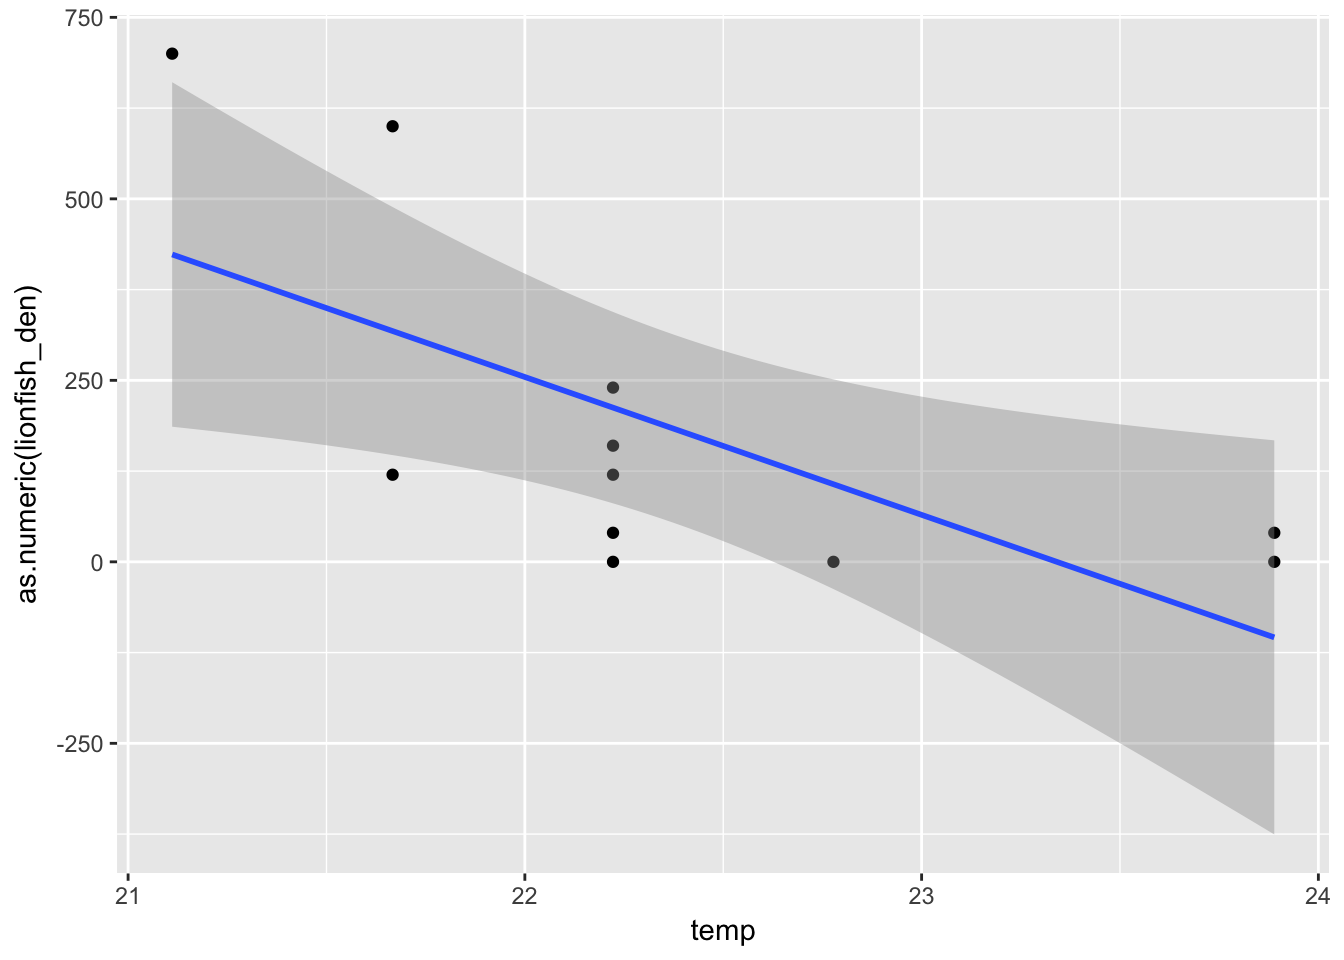
\includegraphics{Darwin_correlation_final_files/figure-latex/unnamed-chunk-6-1.pdf}

\begin{Shaded}
\begin{Highlighting}[]
\KeywordTok{ggsave}\NormalTok{(darwin, }\DataTypeTok{plot =}\NormalTok{ darwin_corr, }\DataTypeTok{device =} \StringTok{"eps"}\NormalTok{, }\DataTypeTok{path =} \StringTok{"~/Desktop/Lionfish"}\NormalTok{)}
\end{Highlighting}
\end{Shaded}

\begin{verbatim}
## Saving 6.5 x 4.5 in image
\end{verbatim}


\end{document}
